\documentclass[conference]{IEEEtran}

\usepackage{datetime}
\usepackage{cite}
\usepackage[pdftex]{graphicx}
\usepackage{epstopdf}
\usepackage[utf8]{inputenc}
\usepackage{amsfonts}
\usepackage{amssymb}
\usepackage{graphicx}
\usepackage{tikz}
\usepackage{float}
\usepackage{color}
\usepackage{subfig}

\hyphenation{}

\newcommand{\xcloud}{x-cloud }

\begin{document}

\title{\xcloud challenges}


% author names and affiliations
% use a multiple column layout for up to three different
% affiliations
\author{\IEEEauthorblockN{Michael Shell}
\IEEEauthorblockA{School of Electrical and\\Computer Engineering\\
Georgia Institute of Technology\\
Atlanta, Georgia 30332--0250\\
Email: http://www.michaelshell.org/contact.html}
\and
\IEEEauthorblockN{Homer Simpson}
\IEEEauthorblockA{Twentieth Century Fox\\
Springfield, USA\\
Email: homer@thesimpsons.com}
\and
\IEEEauthorblockN{James Kirk\\ and Montgomery Scott}
\IEEEauthorblockA{Starfleet Academy\\
San Francisco, California 96678-2391\\
Telephone: (800) 555--1212\\
Fax: (888) 555--1212}}


\maketitle


\begin{abstract}
%\boldmath
The abstract goes here.
\end{abstract}

\IEEEpeerreviewmaketitle


\section{Introduction}


\begin{figure}[tb]
	\centering
	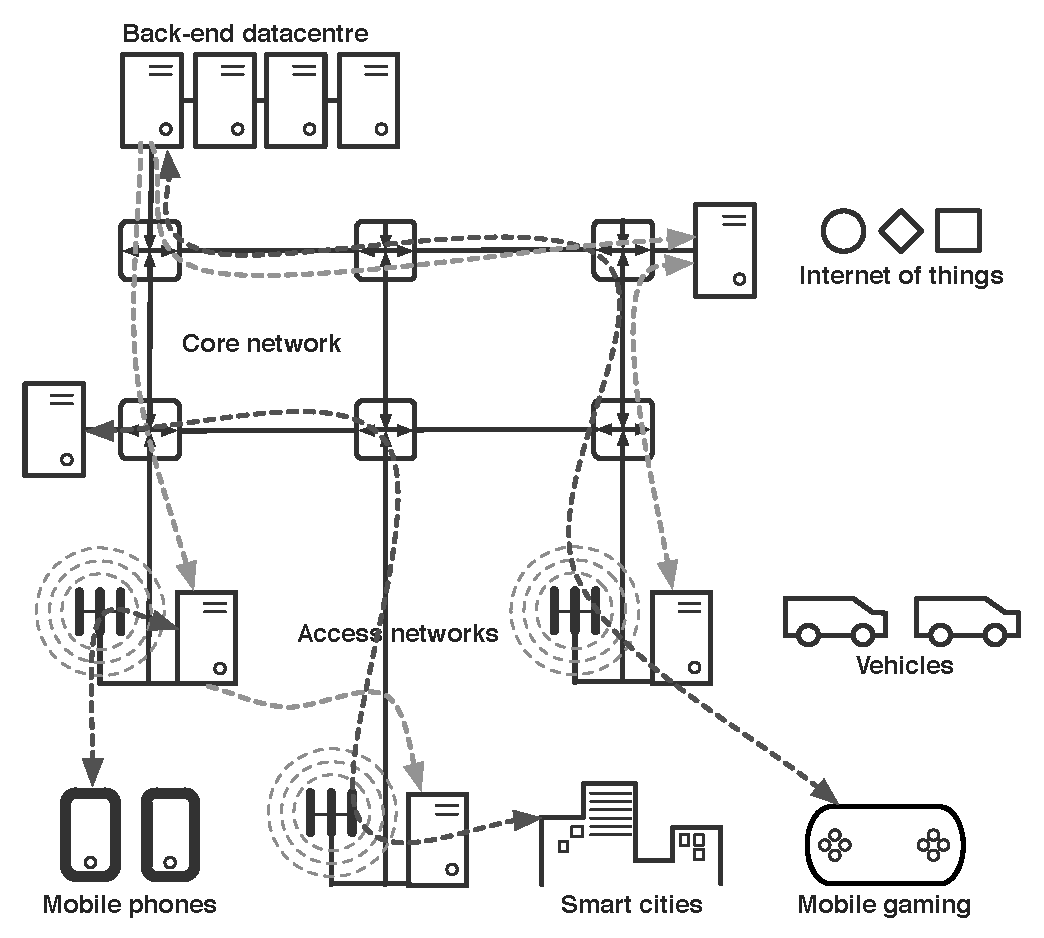
\includegraphics[width=\linewidth]{diagram_overview.pdf} 
	\caption{Omnipresent cloud}
	\label{fig:diagram_overview}
\end{figure}

\section{The case for the \xcloud}

\subsection{The bandwidth case for \xcloud}

\subsection{The latency case for \xcloud}
The intermediate latency between a client and a data-centre is a product of propagation, modulation, and network routing and traffic shaping. Propagation is a clear physical obstacle to reducing latency, and there is very little evidence to suggest that information will propagate faster than $\frac{2}{3}$ of the speed of light, at scale, in the near future. Furthermore, the delay in the backbone network is incurred to the most part by routing. A full point to point network where the propagation speed is the only limit, is not economically viable and would dissolve the fabric of the Internet. As such, we can always expect a certain amount of network contributed latency and jitter. At best, an LTE mobile access network adds about 5 ms of latency \cite{blajic2006latency}. Radio access network latency can be expected to diminish over the next few generations of mobile networks. 

\begin{figure}[tb]
	\centering
	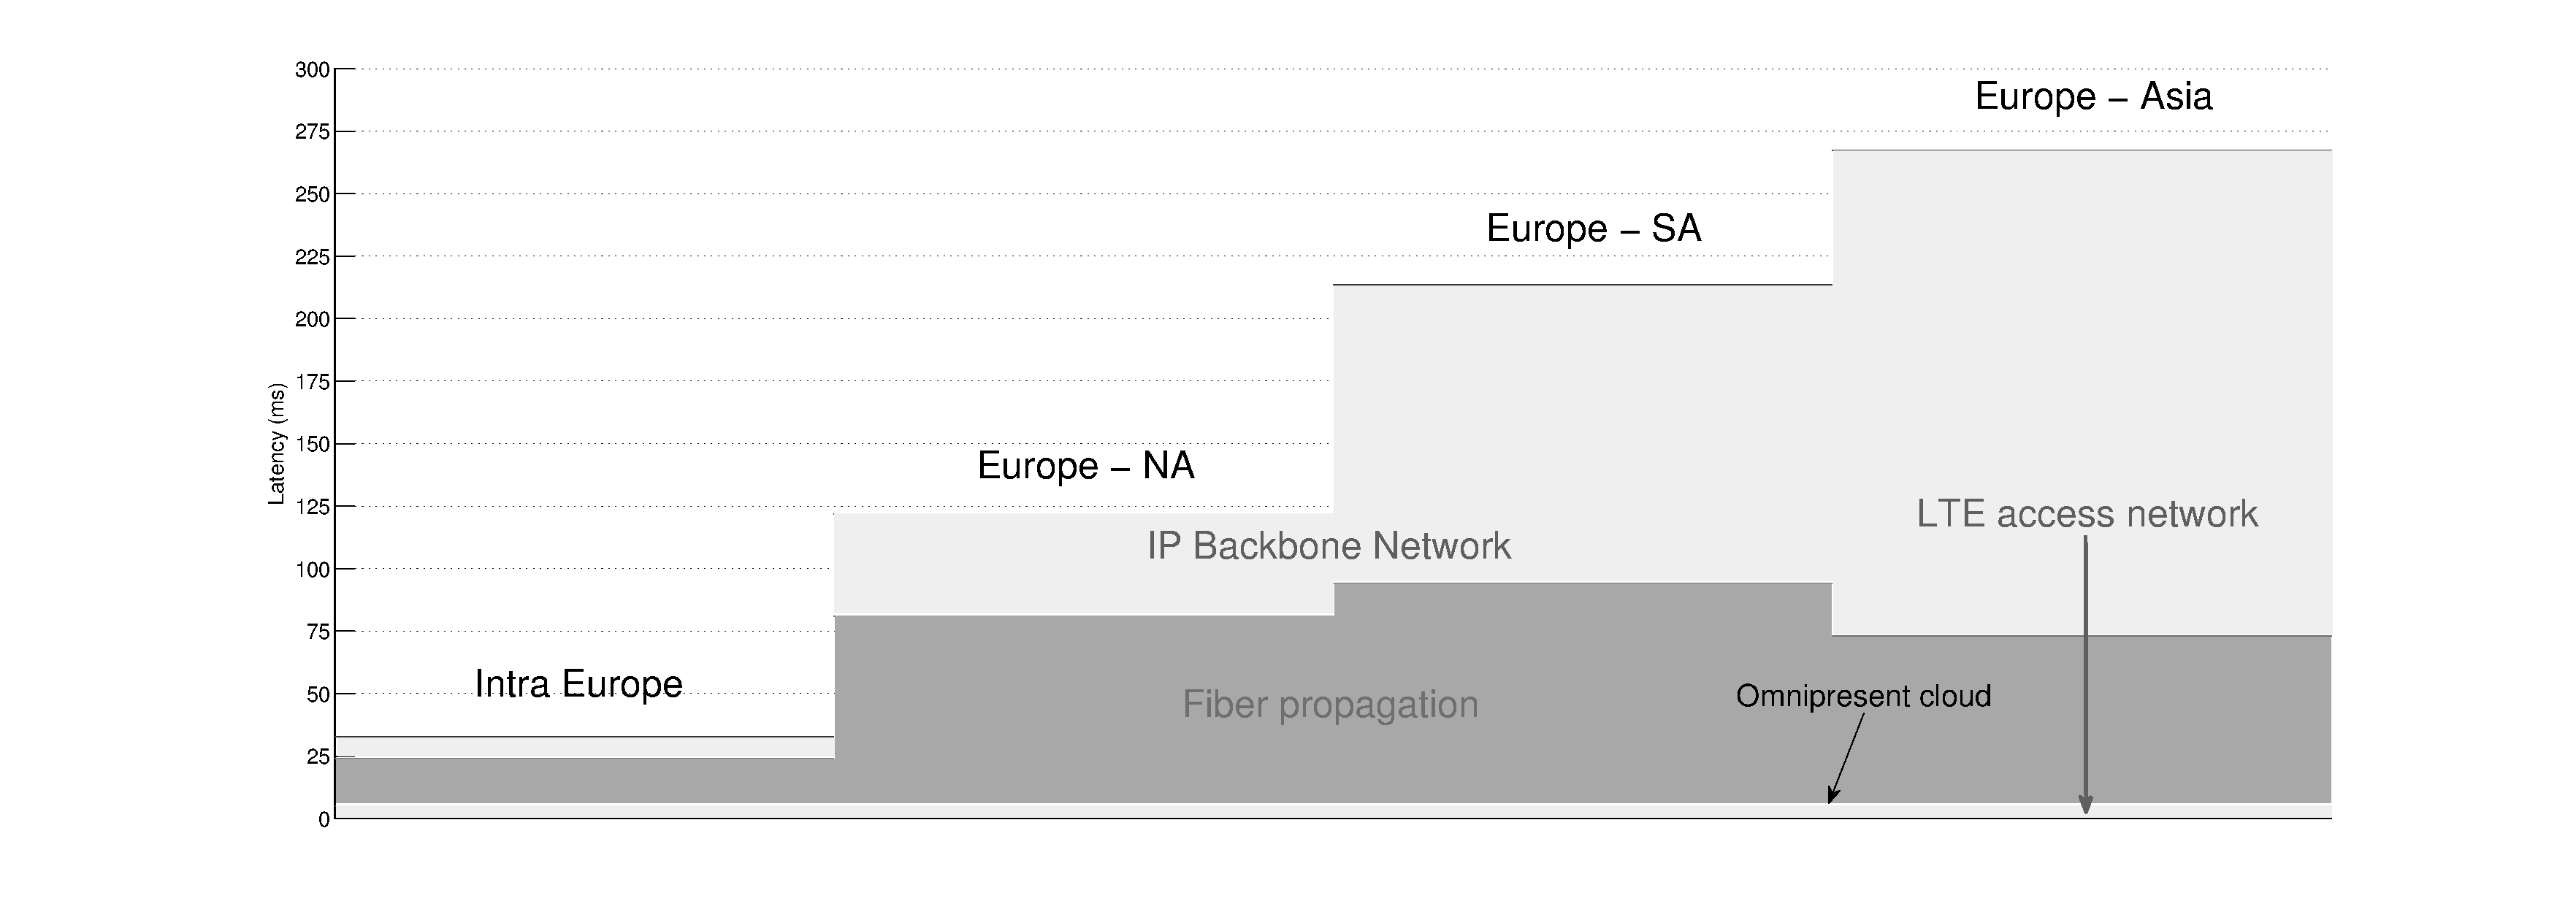
\includegraphics[height=0.12\paperheight]{omni_motivation.pdf} 
	\caption{IP Internet latency in western Europe \cite{BT_IP} over LTE \cite{blajic2006latency}}
	\label{fig:omni_motivation}
\end{figure}

Moving the cloud data centres closer to the IP backbone networks eliminates some of the additive latency on one side of the connection. Doing so, not only eliminate the propagation delay, but will over time, add more complexity to peripheries of the backbone as more severs nodes make their home there. 

The \xcloud remedies this latency challenge in a more sustainable way. By moving compute resources to the mobile networks, IP backbone network propagation and routing delays are eliminate without disrupting the Internet topology. The resulting distributed infrastructure is capable of delivering content and services at latencies less than 10 ms. 

The \xcloud will thus enable latency-sensitive services to be migrated to the cloud, such as, gaming, financial trading, process control, and most real-time human-machine interaction process.

\subsection{The infrastructure case for \xcloud}
Distributed virtualized mobile networks will rely on centralized compute nodes for higher level link management. One node will proposedly host multiple base stations, to which they connect over a network link, much like the Ericsson Radio Dot System \cite{ericsson_dot}, but at a larger scale. The size of these virtualization resource nodes is proportional to the maximum distance they can reside from the radio nodes, given the induced propagation delay. Supposedly these virtualization resource nodes will the placed in the vicinity of the core IP network. The virtualization resource nodes can be seen as to define geographic areas whos boundaries are defined by the reach of the mobile network which it serves. Depending on the level of desired provision and load balancing flexibility, these geographic domains will overlap to varying degrees.

The virtualization resource nodes are conceivably constructed of generic x86 or ARM servers, hosting VMs or containers within which the virtualized mobile network infrastructure is executed. Given the placement of the virtualization resource node, any free or designually excess capacity can be used hist other services.

The the topology is designed to optimize the use of radio resources, the geographic domains which the virtualization resource nodes constitute do not necessarily overlap or map the demographic area which \xcloud services operate.

\section{Simulation model}

\subsection{Python + [NS-3, Omnet, Matlab, Modelica]}

\subsection{Java}

\section{Conclusion}


\bibliographystyle{plain}
\bibliography{references}

\end{document}